\documentclass[a4paper, 12pt]{article}

\usepackage{geometry}
\geometry{left=2cm, right=2cm, top=2cm, bottom=2cm}

\usepackage{cmap}
\usepackage{mathtext} 
\usepackage[T2A]{fontenc}
\usepackage[utf8]{inputenc}
\usepackage[english,russian]{babel}	

\usepackage{amsfonts,amssymb,amsthm,mathtools}
\usepackage{amsmath}
\usepackage{icomma} 

\usepackage{graphicx} 
\graphicspath{{picturies/}}
\usepackage{wrapfig}

\usepackage{array,tabularx,tabulary,booktabs}
\usepackage{longtable}
\usepackage{multirow}

\usepackage{caption}
\captionsetup{labelsep=period}

\renewcommand{\phi}{\varphi}
\newcommand{\eps}{\varepsilon}
\newcommand{\parag}[1]{\paragraph*{#1:}}

\newcounter{Points}
\setcounter{Points}{1}
\newcommand{\point}{\arabic{Points}. \addtocounter{Points}{1}}

\author{Радькин Кирилл, Б01-005}
\date{11.03.22}
\title{Лабораторная работа 4.7.2, Эффект Поккельса.}

\begin{document}
\maketitle

\parag {Цель работы} исследовать интерференцию рассеянного света, прошедшего кристалл; наблюдать изменение характера поляризации света при наложении на кристалл электрического поля.

\parag {В работе используются} гелий-неоновый лазер, поляризатор, кристалл ниобата лития, матовая пластинка, экран, источник высоковольтного переменного и постоянного напряжения, фотодиод, осциллограф, линейка.

\parag{Теоретическая справка} ~

\begin{itemize}
    \item Эффектом Поккельса называется изменение показателя преломления света в кристалле под действием электрического поля, причём это изменение пропорционально напряжённости электрического поля. В первом приближении это изменение считается линейным относительно напряженности.
    
    \item Эффект Поккельса может наблюдаться только в кристаллах, не обладающих центром симметрии. Вследствие линейности эффекта относительно внешнего поля $E$ эл при изменении направления поля на противоположное должен меняться на противоположный
    и знак изменения показателя преломления $\Delta n$. Но в кристаллах с центром симметрии это невозможно, так как оба взаимно противоположных направления внешнего поля физически эквивалентны
    
    \item Выражение для радиуса $m$-нного темного кольца для случая, когда направление анализатора перпендикулярно поляризации лазерного излучения:

    \begin{equation}
        r^2_m = \dfrac{\lambda}{l} \dfrac{(n_0 L)^2}{(n_0 - n_e)m}
    \end{equation}
    
    где: $\lambda$~---~длина волны лазерного излучения, $l$~---~длина кристалла, $n_0$~---~показатель преломления кристалла для случая, когда вектор $\vec{E}$ перпендикулярен оптической оси кристалла $Z$, $n_e$~---~показатель преломления для случая, когда вектор $\vec{E}$ располагается вдоль оси $Z$
\end{itemize}

\parag {Ход работы} ~

\begin{enumerate}
    \item Соберем оптическую схему, включим лазер, получим на экране интерференционную картину
    \item Измерим радиусы темных колец $r(m)$ и расстояние $L$ от середины кристалла до экрана, построим график.

    $L = 76.5$ см

    \begin{tabular}{|c|c|c|c|c|c|c|} \hline
        $r$, см & 2.85 & 3.9 & 4.85 & 5.5 & 6.2 & 6.8 \\ \hline
        $m$ & 1 & 2 & 3 & 4 & 5 & 6 \\ \hline   
    \end{tabular}

    \item Построим график $r^2$ от $m$
    
    \begin{figure}
        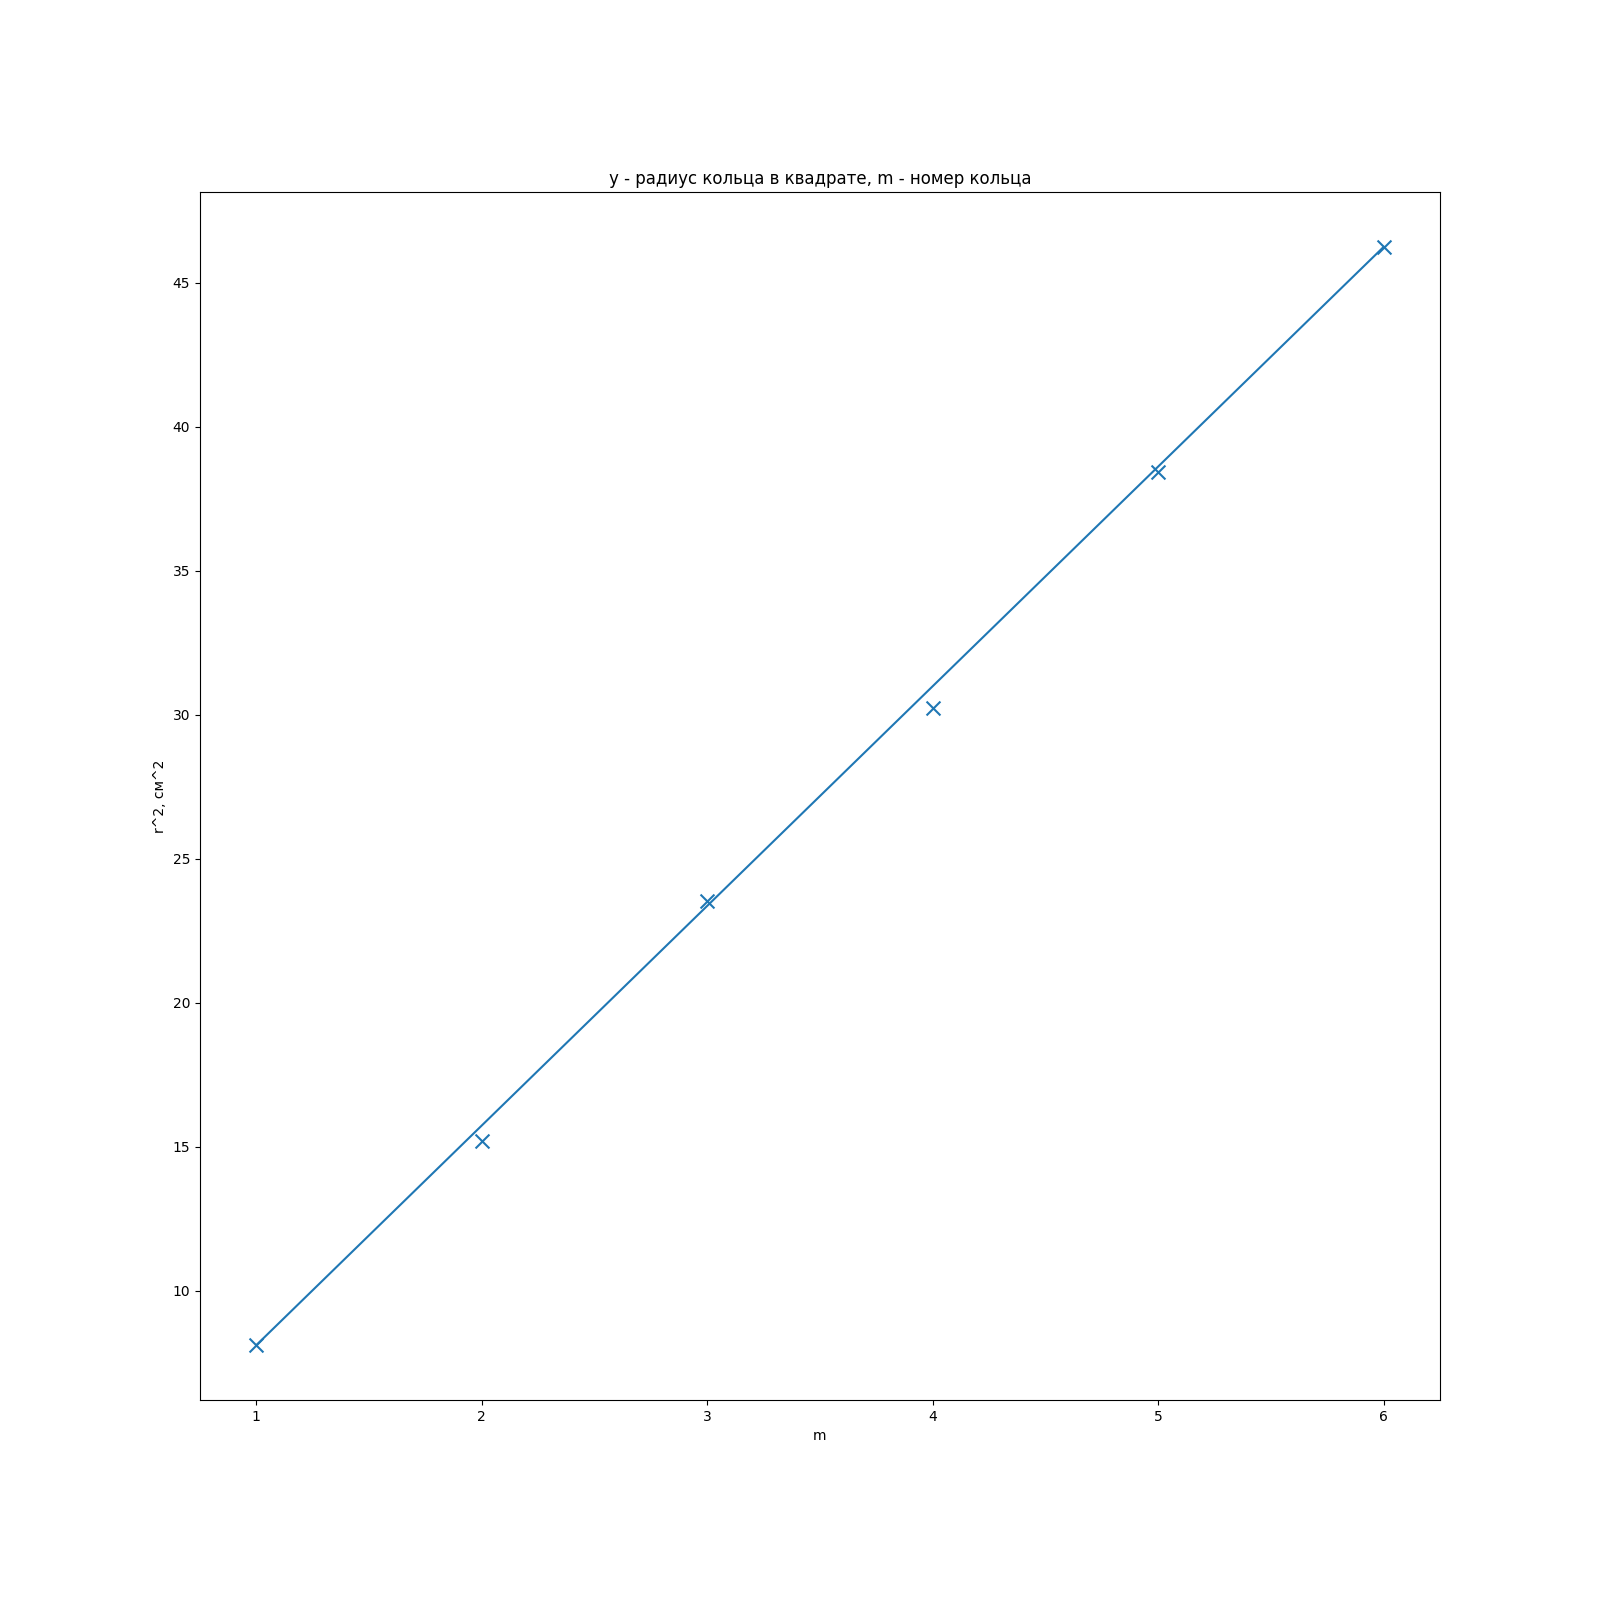
\includegraphics[scale=0.45]{graph1.png}
        \centering
        \caption{$r^2$ от $m$}
        \label{graph1}
    \end{figure}

    По углу наклона прямой определим лучепреломление $n_0 - n_e$ ~

    Необходимые табличные величины: $n_0 = 2.29$, $l = 26$ мм, $\lambda = 0.63$ мкм

    Полученный угол наклона: $k = 7.62 \pm 0.67$ $см^2$, тогда величина $n_0 - n_e = 0.097 \pm 0.011$

    \item Подключим блок питания. Уберем матовую пластину, на экране появляется пятно. С увеличением напряжения яркость пятна увеличивается, достигает максимума при $U = U_{\lambda / 2} = 300$ В.
    
    \item Подадим на кристалл напряжение $U = \dfrac{U_{\lambda / 2}}{2}$ и убедимся, что поляризация на выходе кристалла получается круговой.

    \item Установим вместо экрана фотодиод и подклюич осциллограф
    
    \item Определим по осциллографу полуволновое напряжение, соответствующее максимуму и минимуму сигнала на осциллограмме: $U_{\lambda / 2} = 474$ В.
    
    \item Зафиксируем фигуры Лиссажу для напряжений $U_{\lambda / 2}, U_{\lambda}, U_{3\lambda / 2}$
    
    \begin{figure}
        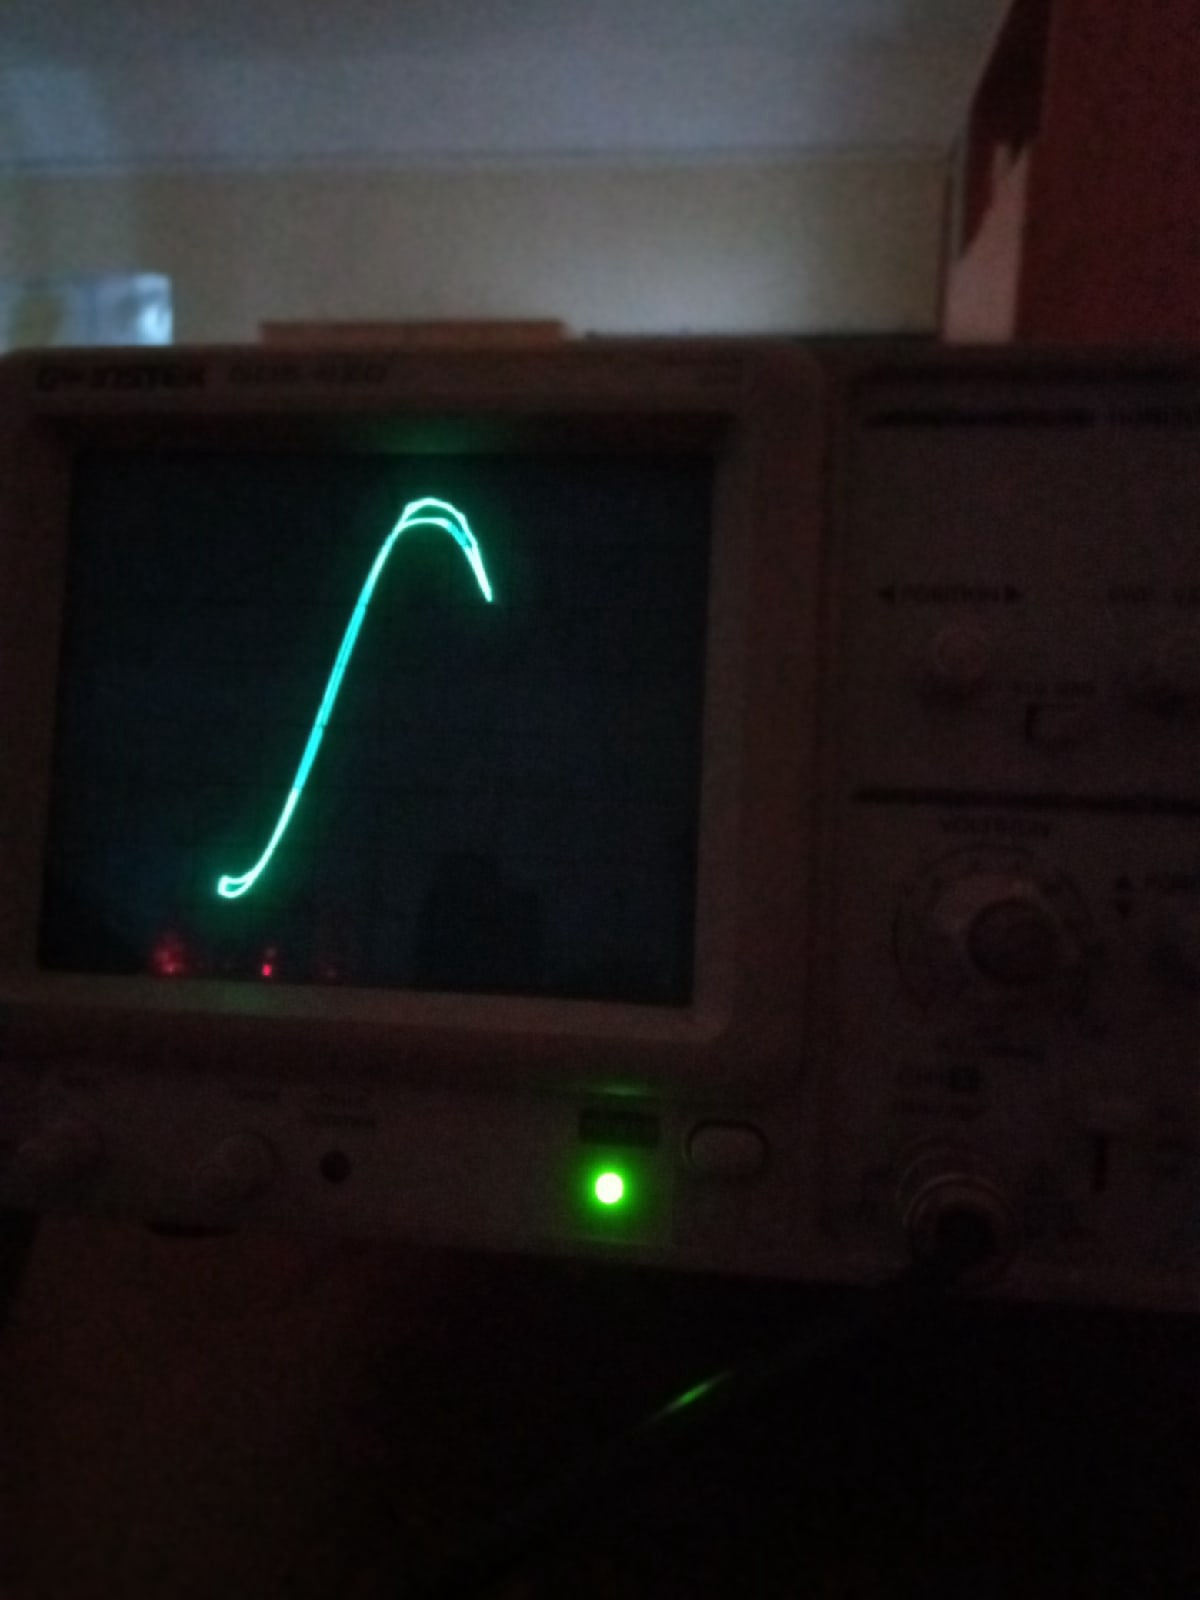
\includegraphics[scale=0.3]{pic1.jpg}
        \centering
        \caption{Осцилограмма $U_{\lambda / 2}$}
        \label{pic1}
    \end{figure}

    \begin{figure}
        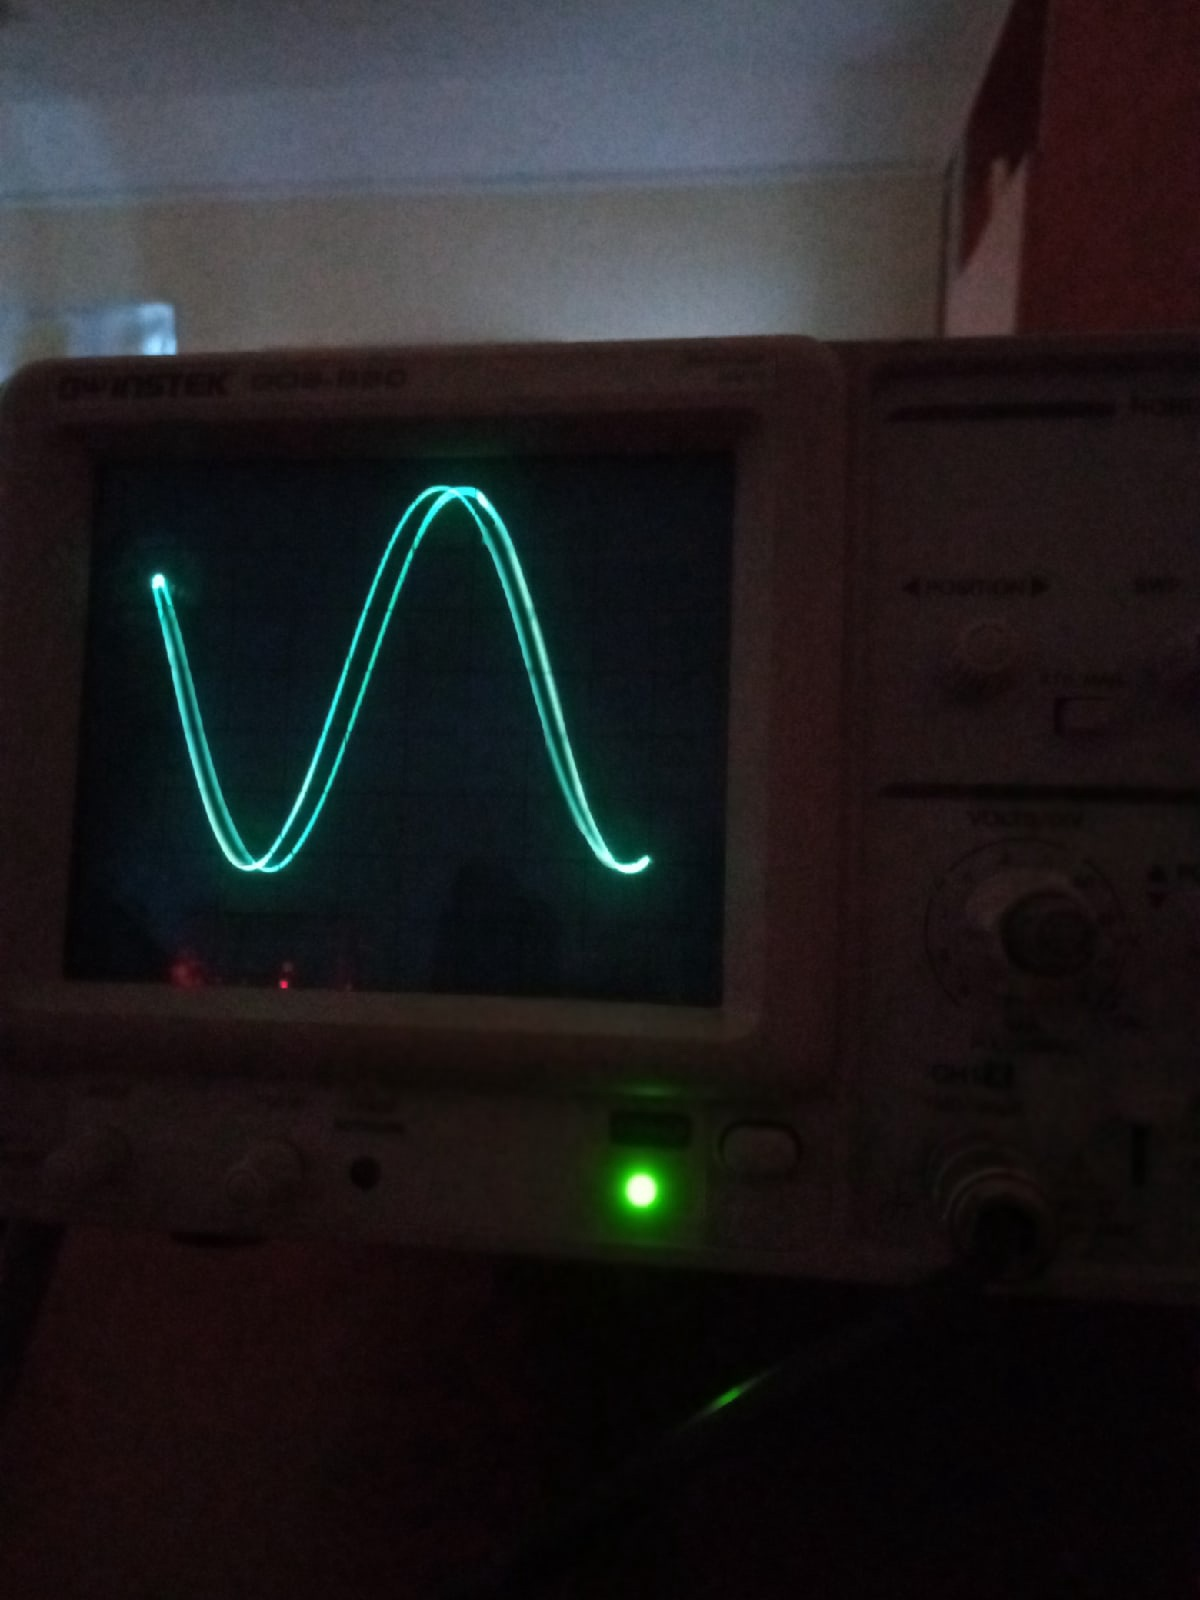
\includegraphics[scale=0.3]{pic2.jpg}
        \centering
        \caption{Осцилограмма $U_{\lambda}$}
        \label{pic2}
    \end{figure}

    \begin{figure}
        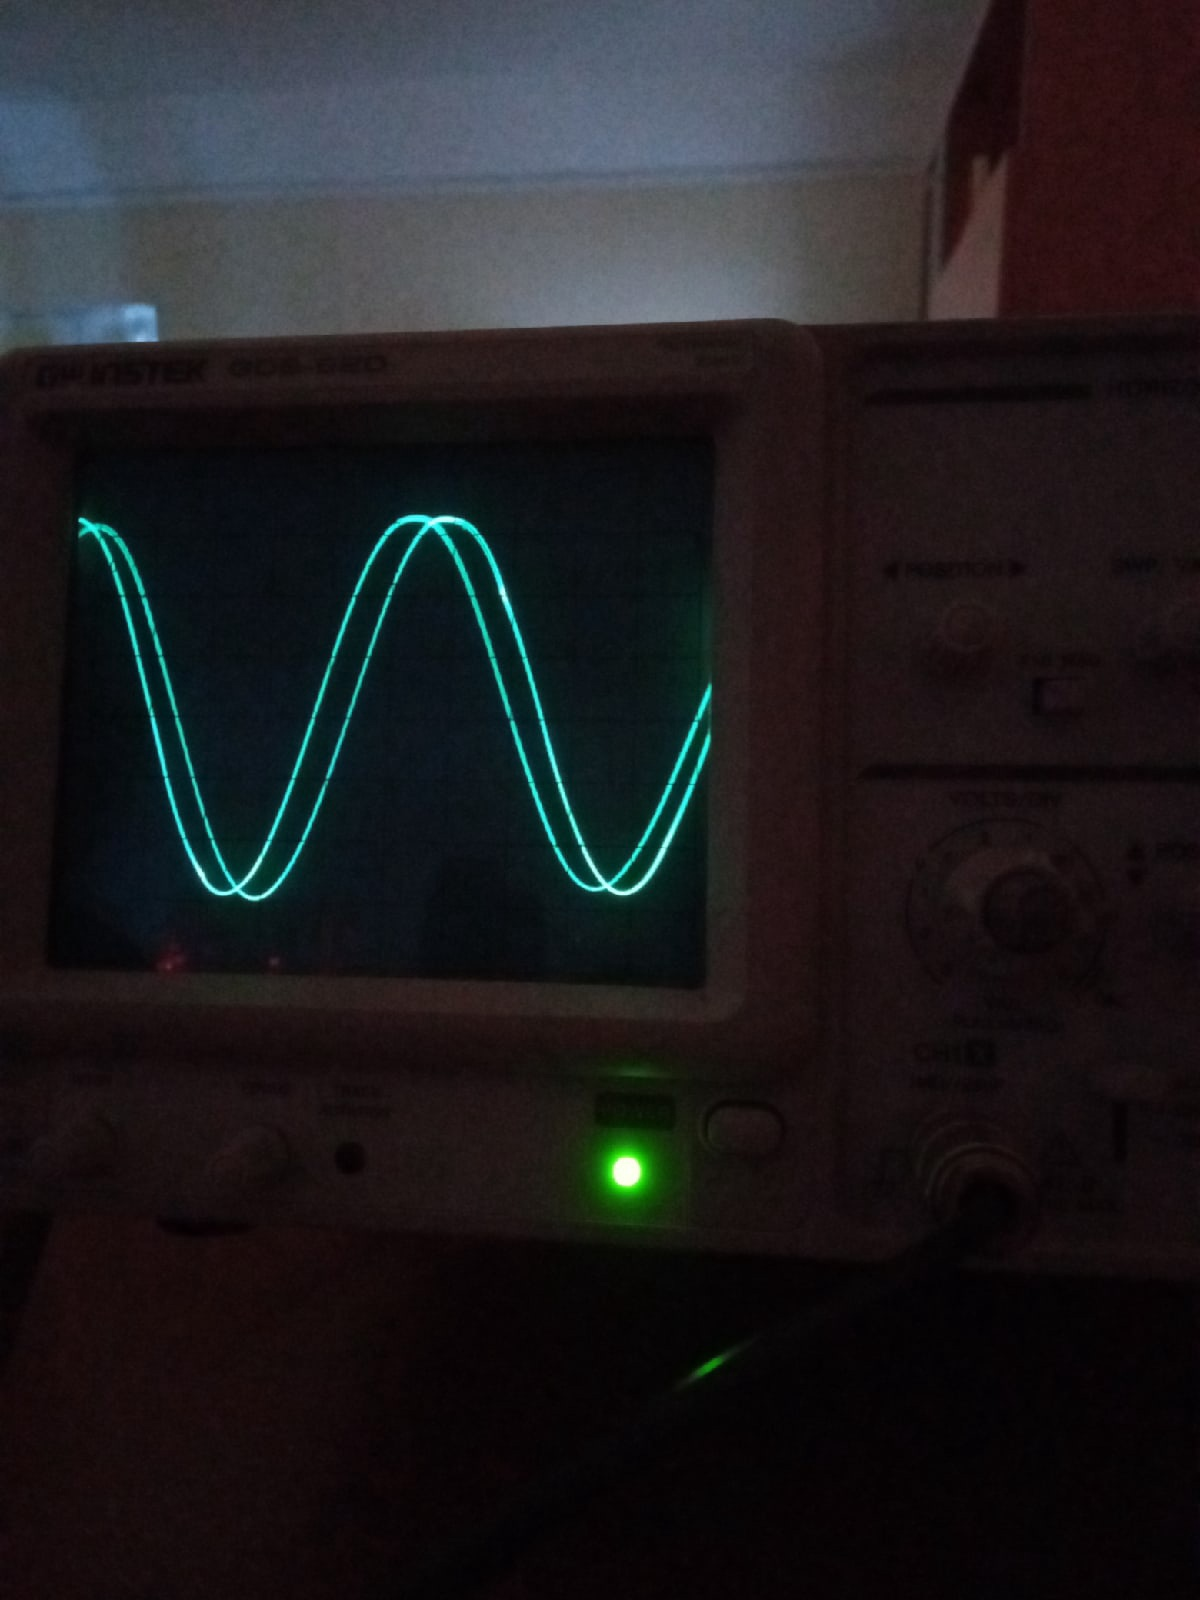
\includegraphics[scale=0.3]{pic3.jpg}
        \centering
        \caption{Осцилограмма $U_{3\lambda / 2}$}
        \label{pic3}
    \end{figure}
\end{enumerate}

\end{document}